\newif\ifpdf
  \ifx\pdfoutput\undefined
  \pdffalse
\else
  \pdftrue
\fi

\documentclass[12pt,twoside]{book}

%%% define a macro \ifpdf para compila��o condicional -- PDF ou
%%% DVI/PS.


\usepackage[ruled]{algorithm2e}
\renewcommand{\listalgorithmcfname}{Lista de Algoritmos}%
\renewcommand{\algorithmcfname}{Algoritmo}%

\usepackage[english,brazil]{babel}
\usepackage{subfigure}

%%% acentua��o
\usepackage[latin1]{inputenc}


%%% bibliografia
%\usepackage{chicago}
\usepackage{natbib}

\usepackage{latexsym}


\usepackage{setspace}


\usepackage{xspace}


\usepackage{acronym}
%%% referencias com p�gina \vref
\usepackage[brazil]{varioref}

%%% identa primeiro par�grafo
\usepackage{indentfirst}

%%% figuras um ao lado do outro
\usepackage{subfigure}


%%% definir t�tulos de se��o
\usepackage[sf,sl,outermarks]{titlesec}


%%% boxes
\usepackage{fancybox}
\usepackage{fancyvrb}
\usepackage{color}

\ifpdf
%%% somente na vers�o PDF

%%% Para inclus�o de gr�ficos
%\usepackage[pdftex]{graphicx}
\usepackage{graphicx}

%%% dimens�es do documento
\usepackage[pdftex]{geometry}
  \geometry{a4paper,left=3cm,right=2cm,top=2.0cm,bottom=2cm,twoside}

%%% cria links no arquivo .pdf
%%% comentar as linhas na vers�o para impressao
\usepackage[pdftex,pdfpagelabels,pagebackref]{hyperref}
%\usepackage{hyperref}


%%% propriedades do arquivo .pdf
\hypersetup{
    pdftitle = {},
    pdfsubject = {},
    pdfkeywords = {},
    pdfauthor = {}
    }



\else
%%% somente na vers�o DVI/PS

%%% Para inclus�o de gr�ficos
\usepackage[dvips]{graphicx}

%%% dimens�es do documento
\usepackage[dvips]{geometry}
 \geometry{a4paper,left=3cm,right=2cm,top=2.0cm,bottom=2cm,twoside}

\usepackage[dvips]{hyperref}

\fi

\hypersetup{colorlinks=true,linkcolor=black,citecolor=black,hypertexnames=false}

%%fonte
\usepackage{bookman}
\usepackage[T1]{fontenc}

%%para os numeros reais
\usepackage{amsfonts}

\DeclareFixedFont{\numberfont}{T1}{phv}{bx}{n}{2cm}

%%% redefine o formato do t�tulo
\titleformat{\chapter}[display]
  {\normalfont\Large\sffamily
  }
  {%\titlerule[3pt]%
   \filright
   \rule[32pt]{.7\linewidth}{4pt}
   \hspace{-11pt}
   \shadowbox{
   \begin{minipage}{.18\linewidth}
     \begin{center}
       \textsc{\Large\chaptertitlename}\\
       \vspace{1ex}
       {\numberfont\color[gray]{0.5} \thechapter}\\
       \vspace{1ex}
     \end{center}
   \end{minipage}}
  }
  {0pt}
  {\filcenter
   \Huge
   }
  [\hfill\rule{.8\textwidth}{0.5pt}\\
     \vskip-1.8ex\hfill\rule{.7\textwidth}{3pt}]


%%% macro para destacar a(s) primeira(s) letra do texto
%%% � necess�rio ter a fonte courier instalada
%
%  um texto do tipo:
%
%  \begin{document}
%    \versal{IN} THE beginning God created the heaven and the earth.  Now the
%    earth was unformed and void, and darkness was upon the face of the
%    deep; and the spirit of God hovered over the face of the waters.
%  \end{document}
%
%  ir� produzir algo como:
%
%  I I\  I THE beginning God  created the heaven and  the earth.
%  I I \ I Now the earth was unformed and void, and darkness was
%  I I  \I upon the face of the deep; and the spirit of God hov-
%  ered over the face of the waters.

%\font\largefont= pzcmi scaled 6500

\newcommand{\versal}[1]{{\noindent
    \setbox0\hbox{\largefont #1 }%
    \count0=\ht0                   % height of versal
    \count1=\baselineskip          % baselineskip
    \divide\count0 by \count1      % versal height/baselineskip
    \dimen1 = \count0\baselineskip % distance to drop versal
    \advance\count0 by 1\relax     % no of indented lines
    \dimen0=\wd0                   % width of versal
    \global\hangindent\dimen0      % set indentation distance
    \global\hangafter-\count0      % set no of indented lines
    \hskip-\dimen0\setbox0\hbox to\dimen0{\raise-\dimen1\box0\hss}%
    \dp0=0in\ht0=0in\box0}}

% BibTeX
\def\BibTeX{{\rm B\kern-.05em{\sc i\kern-.025em b}\kern-.08em
    T\kern-.1667em\lower.7ex\hbox{E}\kern-.125emX}\xspace}

% BibTeX
\def\bibtex{\BibTeX}

% BibView
\def\BibView{{\rm B\kern-.05em{\sc i\kern-.025em b}\kern-.08em
    V\kern-.1667em\hbox{\sc iew}}\xspace}
\def\bibview{\BibView}

% e.g.
\newcommand{\eg}
  {{\em e.g.}\/\xspace}
  
% fitness
\newcommand{\fitness}
  {{\em fitness}\/\xspace}

\begin{document}

\pagestyle{empty}
\pagenumbering{roman}

%%% insere a capa
%%% edite os campos para t�tulo, data, orientador e nome

\newcommand{\titulo}{Monitoramento de Ambientes Internos Utilizando Rob�s M�veis}


\begin{titlepage}


\ \vfill

\begin{center}
\begin{minipage}[c]{12cm}
\begin{center}
\hrulefill\\
\vspace{.5cm} {\Large \titulo}\\
\vspace{1.3cm}
\textbf{\it �gor Assis Braga}\\
\vspace{.5cm}
\hrulefill\\
\end{center}
\end{minipage}
\end{center}

\vfill

\cleardoublepage


\begin{flushright}
\begin{Sbox}
\begin{minipage}{8.5cm}
\footnotesize
SERVI�O DE  P�S-GRADUA��O DO ICMC-USP\\
\\
Data de Dep�sito: \\
\\
Assinatura:\hrulefill
\end{minipage}
\end{Sbox}
\fbox{\TheSbox}
\end{flushright}


\vspace*{2cm}
\begin{center}
{\huge\sf \titulo}\footnote{Trabalho Realizado com
Aux�lio do CNPq}


\vspace*{2cm}

{\it �gor Assis Braga}

\vspace*{2cm}


{\bf Orientadora:}  {\it Prof� Dr� Maria Carolina Monard}

\end{center}

\vspace*{4cm}

\begin{flushright}
\begin{minipage}{10cm}
Monografia apresentada ao Instituto de Ci�ncias Matem�ticas e de
Computa��o - ICMC-USP, para o Exame de Qualifica��o, como parte dos
requisitos necess�rios � obten��o do t�tulo de Mestre em Ci�ncias de
Computa��o e Matem�tica Computacional.
\end{minipage}
\end{flushright}

\vspace*{2cm}
\begin{center}
\textbf{USP - S�o Carlos \\dezembro/2008}
\end{center}
\cleardoublepage



\end{titlepage}


\pagestyle{plain}


\onehalfspacing

%%% insere o resumo

%==========================================================
% Resumo
% 
% Autor
% Heitor Luis Polidoro
% 
% Orientador
% Prof. Dr. Denis Fernando Wolf
%==========================================================

\pagestyle{chapterst}

\chapter*{Resumo}
\label{Resumo}
A rob�tica m�vel � uma �rea de pesquisa que est� obtendo grande aten��o da comunidade cient�fica. O desenvolvimento de rob�s m�veis aut�nomos, que sejam capazes de interagir com o ambiente, aprender e de tomar decis�es corretas para que suas tarefas sejam executadas com �xito � o maior desafio em rob�tica m�vel. O desenvolvimento destes sistemas inteligentes e aut�nomos consiste em uma �rea de pesquisa multidisciplinar, considerada recente e extremamente promissora que envolve: intelig�ncia artificial, aprendizado de m�quina, estima��o estat�stica e sistemas embarcados, por exemplo. Dentro desse contexto, esse trabalho aborda o problema de navega��o e monitoramento de ambientes utilizando rob�s m�veis. Dado uma representa��o do ambiente (mapa topol�gica) e uma lista com urg�ncias de cada uma das regi�es do mapa, o rob� deve estimar qual o percurso mais eficiente para monitorar esse ambiente. Uma vez que a urg�ncia de cada regi�o n�o visitada aumenta com o tempo, o trajeto do rob� deve-se adaptar a essas altera��es. Entre as diversas aplica��es pr�ticas desse tipo de algoritmo, destaca-se o desenvolvimento de sistemas de seguran�a m�veis inteligentes. Experimentos com diferentes algoritmos em diferentes ambientes s�o apresentados.

\cleardoublepage

\tableofcontents
\addcontentsline{toc}{section}{Sum�rio}
\cleardoublepage

\listoffigures
\addcontentsline{toc}{section}{Lista de Figuras}
\cleardoublepage

\listoftables
\addcontentsline{toc}{section}{Lista de Tabelas}
\cleardoublepage


%\input{acron}
%\addcontentsline{toc}{section}{Lista de Abreviaturas}
%\cleardoublepage

\listofalgorithms
\addcontentsline{toc}{section}{Lista de Algoritmos}
\cleardoublepage




%%% inserir resumo
%%==========================================================
% Resumo
% 
% Autor
% Heitor Luis Polidoro
% 
% Orientador
% Prof. Dr. Denis Fernando Wolf
%==========================================================

\pagestyle{chapterst}

\chapter*{Resumo}
\label{Resumo}
A rob�tica m�vel � uma �rea de pesquisa que est� obtendo grande aten��o da comunidade cient�fica. O desenvolvimento de rob�s m�veis aut�nomos, que sejam capazes de interagir com o ambiente, aprender e de tomar decis�es corretas para que suas tarefas sejam executadas com �xito � o maior desafio em rob�tica m�vel. O desenvolvimento destes sistemas inteligentes e aut�nomos consiste em uma �rea de pesquisa multidisciplinar, considerada recente e extremamente promissora que envolve: intelig�ncia artificial, aprendizado de m�quina, estima��o estat�stica e sistemas embarcados, por exemplo. Dentro desse contexto, esse trabalho aborda o problema de navega��o e monitoramento de ambientes utilizando rob�s m�veis. Dado uma representa��o do ambiente (mapa topol�gica) e uma lista com urg�ncias de cada uma das regi�es do mapa, o rob� deve estimar qual o percurso mais eficiente para monitorar esse ambiente. Uma vez que a urg�ncia de cada regi�o n�o visitada aumenta com o tempo, o trajeto do rob� deve-se adaptar a essas altera��es. Entre as diversas aplica��es pr�ticas desse tipo de algoritmo, destaca-se o desenvolvimento de sistemas de seguran�a m�veis inteligentes. Experimentos com diferentes algoritmos em diferentes ambientes s�o apresentados.

%
%\newpage

%%% corpo do texto


\pagenumbering{arabic}

%%% inclua os seu arquivos a partir daqui

%==========================================================
% Capitulo 1: Introducao.
% 
% Autor
% Heitor Luis Polidoro
% 
% Orientador
% Prof. Dr. Denis Fernando Wolf
%==========================================================

\pagestyle{chapterst}

\chapter{Introdu��o}
\label{introducao}

\section{Contextualiza��o}
\label{contextualizacao}
Os rob�s s�o uma tecnologia utilizada para auxiliar ou substituir o homem em tarefas em ambientes insalubres, como fundo do mar, inc�ndios, desarmamento de bombas, �reas com contamina��o radioativa ou com gases t�xicos, em tarefas repetitivas como uma linha de produ��o industrial, em tarefas que o ser humano n�o � capaz de executar, ou tarefas sem valor intelectual.

Entre todas essas diversas aplica��es da rob�tica m�vel, pode-se citar o rob� Sojourner (Figura \subref{fig:sojourner}) da NASA, que explorou e enviou fotos e outras muitas informa��es do planeta Marte para a Terra \cite{NASA}, e o rob� desenvolvido pela universidade Camegie Mellon, chamado Groundhog, que explora minas abandonadas, que al�m do risco de desabamento, em muitos casos tamb�m cont�m gases t�xicos \cite{Thrun2004}.

Dentre as muitas defini��es de rob� podemos destacar:
\begin{itemize}
	\item Dispositivo ou m�quina que realiza fun��es normalmente associadas a seres humanos \cite{Medeiros1998};
	\item M�quinas que, al�m de serem capazes de reproduzir tarefas	e movimentos impl�citos em sua contru��o, complementam a parte mec�nica com dispositivos eletr�nicos inteligentes \cite{Medeiros1998};
	\item Um �rg�o mec�nico vers�rio equipado com atuadores e sensores sob o controle de um sistema computacional \cite{Latombe1991};
	\item Simplesmente um agente artificial e ativo cujo ambiente � o mundo f�sico \cite{Russell2003};
\end{itemize}

Inicialmente, os rob�s foram utilizados para automa��o industrial, presos em posi��es espec�ficas na linha de montagem, os bra�os rob�ticos podem mover-se a uma grande velocidade e precis�o para realizar tarefas repetitivas. Gra�as a essa precis�o sobre-humana � poss�vel a constru��o de \textit{Notebooks} e telefones port�teis. No entranto esses rob�s sofrem uma fundamental disvantagem: Falta de mobilidade. Um manipulador fixo tem alcance limitado que depende de onde foi colocado. Rob�s m�veis, entretando, s�o capazes de locomoverem-se pela f�brica \cite{Siegwart2004}. Mas com a evolu��o tecnol�gica os rob�s passaram a ser utilizados em outras �reas como: medicina de precis�o, ambientes perigosos, ambientes insalubres, na �rea de entretenimento, servi�os dom�sticos, etc. Nesse contexto surgiram as pesquisas para o desenvolvimento de rob�s m�veis aut�nomos, que sejam capazes de atuar em ambientes reais e reagir a situa��es desconhecidas de forma inteligente \cite{Thrun2002}.

A comunidade cient�fica aposta que sistemas rob�ticos estejam cada vez mais presentes em nossa vida cotidiana, o que torna esta �rea de pesquisa extremamente promissora e desafiadora. Segundo \cite{Gates2007}, estamos entrando numa nova era da computa��o, comparando os rob�s industriais com os mainframes de antigamente, e prev� que existir� um rob� em cada casa no futuro.

A rob�tica consiste em uma �rea multidisciplinar de pesquisa, envolvendo desde elementos de engenharia mec�nica, el�trica, computa��o at� �reas de humanas como psicologia e estudos do comportamentais. O que diferencia a rob�tica m�vel de outras �reas de pesquisa em rob�tica, � a sua �nfase nos problemas relacionados com locomo��o em ambientes complexos, que se modificam dinamicamente, compostos tanto por obst�culos fixos quanto por obst�culos m�veis. Para operar nesses ambientes o rob� deve ser capaz de adquirir e utilizar conhecimento sobre o ambiente, tais como: estimar posi��es dentro do ambiente (sua posi��o, de um obst�culo, de um \textit{landmark}, de uma meta, et al.), reconhecer obst�culos, e responder em tempo real �s situa��es que podem ocorrer nesses ambientes. As tarefas de perceber o ambiente, se localizar no ambiente e mover-se pelo ambiente s�o problemas fundamentais da rob�tica m�vel \cite{Heinen2002}. 

A rob�tica m�vel, al�m de ser uma �rea de grande potencial cient�fico, empresas de tecnologia est�o cada vez mais investindo em produtos. Como por exemplo o desenvolvimento de rob�s que realizam trabalhos dom�sticos autonomamente,  entre os quais o aspirador de p� Roomba da IRobot \cite{IRobot} (Figura \subref{fig:roomba}) e o rob� cortador de grama Robomow (Figura \subref{fig:robomow}) da Friendly Robotics \cite{FriendlyRobotics}. Ambos apresentam sucesso comercial. 

\begin{figure}[ht]
  \centering
	\subfigure[Sojourner]{
    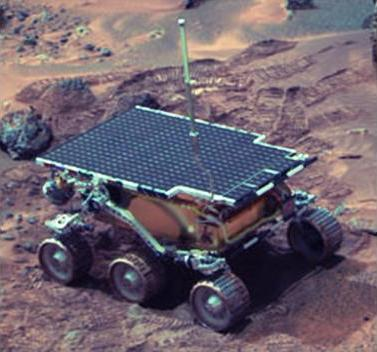
\includegraphics[width=0.4\textwidth]{../imagens/sojourner.jpg}
		\label{fig:sojourner}}	
	\subfigure[Roomba]{
	  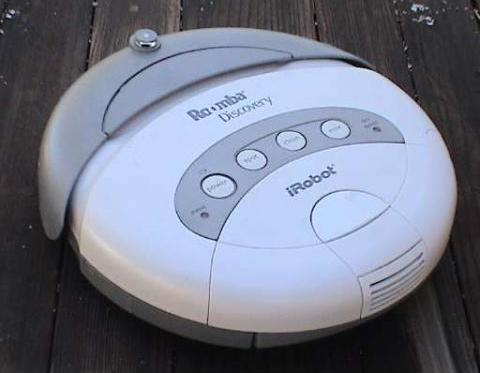
\includegraphics[width=0.4\textwidth]{../imagens/roomba.jpg}
		\label{fig:roomba}}
	\subfigure[Robomow]{
	  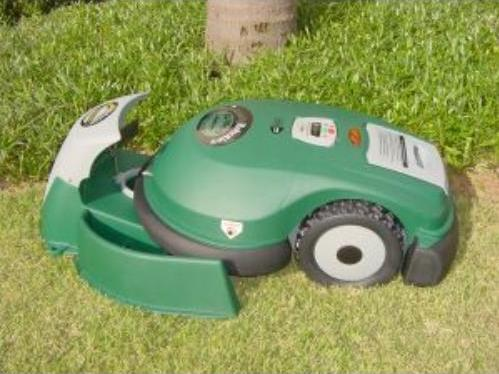
\includegraphics[width=0.4\textwidth]{../imagens/robomow.jpg}
		\label{fig:robomow}}
	\label{fig:exemplo_de_robos}
	\caption{Exemplos de rob�s.}
\end{figure}


Rob�s m�veis podem ser classificados como: homan�ides, com pernas e com rodas. Rob�s com rodas s�o mais simples de serem constru�dos e mais f�ceis de controlas, as rodas permitem uma maior praticidade de locomo��o e d�o um maior suporte est�tico ao rob� \cite{Russell2003}. A autonomia de rob�s m�veis � essencial em ambientes remotos, tais como planetas distantes, onde o tempo de comunica��o entre o rob� e seu operador n�o permite seja grande o suficiente para prejudicar deci�es em tempo real.

Normalmente, a navega��o � a principal tarefa a ser executada por um rob� m�vel. Esta consiste nos passos de localiza��o do rob� no ambiente, planejamento de um caminho entre a posi��o inicial e o destino final e a execu��o do movimento pelo caminho planejado. Esta tarefa pode ser mais, ou menos, complexa, depende do ambiente em que o rob� se encontra \cite{Pedrosa2001}

A proposta desse projeto � desenvolver uma aplica��o de rob�tica m�vel para o monitoramento de ambientes internos, onde normalmente, nesses ambientes, existem regi�es cr�ticas que possuem prioridades distintas para serem monitoradas. A prioridade (urg�ncia) da visita de cada uma dessas regi�es aumenta conforme o tempo passa e essa regi�o n�o � visitada. Ao ser visitada, a urg�ncia de uma determinada regi�o �, ent�o, zerada. Para a solu��o do problema descrito anteriormente, sup�es-se que o rob� tenha uma descri��o do ambiente em que atua (mapa). 

Na literatura, um problema semelhante que vem sendo estudando h� muitos anos � o Problema do caixeiro-viajante da classe de problemas de roteamento de n�s, onde o caixeiro deve, dado um conjunto de cidades, partir de uma cidade base, visitar as outras somente uma vez e retornar � base \cite{Arenales2007}. 

\section{Motiva��o}
\label{motivacao}
O desenvolvimento de sistemas para controlar rob�s m�veis aut�nomos tem se mostardo um grande desafio para a Intelig�ncia Artificial. Diferentes abordagens de sistema de controle para rob�s m�veis aut�nomos vem sendo utilizadas em diversar �reas de pesquisa. Existem diversas aplica��es poss�veis para rob�s m�veis. Transporte, vigil�ncia, inspe��o, limpeza, explora��o, aux�lio a deficientes f�sicos, et al. \cite{Heinen2002}.

A motiva��o deste projeto de mestrado � desenvolver um sistema de monitoramento de ambientes internos. Existem diversas aplica��es pr�ticas para esse tipo de aplica��o. Dentre elas, pode-se citar o desenvolvimento de um rob� vigia que monitora um ambiente, dando �nfase para �reas de maior import�ncia. Outro exemplo consiste em um rob� que monitora a temperatura e umidade de ambientes onde esse fator � cr�tico. Ou at� mesmo um rob� para entregar rem�dios a pacientes em um hospital.

Durante o ano de 2006 foi iniciado o projeto de mesmo prop�sito. Foram desenvolvidos algoritmos de modo imp�rico, sem base cient�fica, por�m o projeto serviu para formar uma base de conhecimento para poder, neste projeto de mestrado, aprofundar no assunto para determinar, de modo cient�fico, o algoritmo ou estrat�gia mais eficiente para o monitoramento de ambientes internos utilizando rob�s m�veis.

\section{Objetivo}
\label{objetivo}
Esse projeto tem como objetivo o desenvolvimento e compara��o entre estrat�gias e algoritmos para determinar uma seq��ncia de �reas a serem visitadas em ambientes internos com a finalidade de monitoramento desses ambientes utilizando um rob� m�vel. O problema a ser resolvido consiste na divis�o de um ambiente previamente conhecido em �reas de interesse. A cada uma dessas �reas � atribu�do um valor (peso) referente a sua import�ncia de monitoramento. A prioridade com que o rob� deve visitar determinadas �reas � calculada com base na import�ncia dessas �reas e no tempo decorrido desde a sua �ltima visita. �reas de maior import�ncia devem ser visitadas mais freq�entemente. 

As avalia��es consistem na compara��o dos algoritmos e estrat�gias. Ser�o utilizados dois crit�rios de compara��o, um crit�rio comparando a freq��ncia relativa de cada sala com sua prioridade relativa, onde o melhor resultado � aquele em que a freq��ncia relativa se aproximar mais da prioridade relativa. O segundo crit�rio � um gr�fico mostrando a progress�o da somat�ria dos graus de urg�ncia de todas as salas.

%\section{Organiza��o da Monografia}
%\label{organizacao_monografia}
%Organiza��o da monografia.

\chapter{Minera��o de Textos}
\label{cap:textmining}

\section{Etapas da Minera��o de Textos}

\subsection{Pr�-processamento}

\subsection{Extra��o de Padr�es}

\subsection{Outras Etapas}



\section{Tarefas de Minera��o de Textos}

\subsection{Classifica��o}

\subsection{Outras Tarefas}
\chapter{Aprendizado Semi-supervisionado Multivis�o em Textos}
\label{cap:semi}

\section{Aprendizado Semi-supervisionado}

\section{O Algoritmo \cotraining}

\section{Extra��o de Vis�es em Textos}
\chapter{Extra��o de Terminologia}
\label{cap:term}

\chapter{Ferramentas de Apoio}
\label{cap:tools}

\section{\pretext -- um Pr�-processador de Textos}

\section{O Ambiente para Aprendizado \discover}

\section{Ferramentas para Extra��o de Terminologia}
\chapter{Plano de Trabalho}
\label{cap:plano}

\section{Metodologia}

\section{Avalia��o}

\subsection{Experimentos}

\section{Requisitos, Atividades e Cronograma}

\subsection{Requisitos do Programa}

\subsection{Atividades Futuras e Cronograma}

\chapter{Resultados Esperados}
\label{cap:conclusao}


\appendix
\bibliographystyle{apalike}

%%% arquivo .bib
\bibliography{main}
\addcontentsline{toc}{chapter}{Refer�ncias}


% Set the ending of a LaTeX document
\end{document}
